\documentclass{article}
\usepackage[margin=1cm]{geometry}
\usepackage{tikz}
\usepackage{graphicx}
\usepackage{xparse}
\usepackage[sfdefault,condensed]{universalis}
\usepackage{keyval}
\usepackage{xstring}
\usetikzlibrary{positioning}

\makeatletter
\NewDocumentCommand{\gurps@xstrut}{}{\rule[-.4\baselineskip]{0pt}{1.2\baselineskip}}
\NewDocumentCommand{\gurps@wc@attr}{mm}{\mbox{\gurps@xstrut \textbf{#1}~#2}}

\def\gurps@wc@weaponpic{}

% Sorts tikz preamble. Takes two arguments: type and number of lines.
\NewDocumentCommand{\gurps@wctemplate@preamble}{m}{
  \def\ro{0.15}
  \pgfmathsetmacro\xmax{8}
  \pgfmathsetmacro\ymax{\xmax/1.618/2}
  \pgfmathsetmacro\ymaxminusmargin{\ymax cm - 12pt}
  % \pgfmathsetmacro\xlineskip{\ymax/#2}
  \def\xstrut{\rule[-.4em]{0.0pt}{1.2em}}
  \def\xsep{\discretionary{%
      \xstrut%
    }{}{%
      \rule{1ex}{0pt}%
      \rule[-.4em]{0.3pt}{1.2em}%
      \rule{1ex}{0pt}}}
  % \def\xsep{\discretionary{X}{Y}{Z}}
  \coordinate (topcorner) at (\xmax,\ymax);
  \coordinate (picture top right) at (\ymax,\ymax);
  \coordinate (origin) at (0, 0);

  \draw[use as bounding box, draw=none] (origin) -- (topcorner);
  \draw[dotted] (origin) rectangle (topcorner);
  \coordinate [above right = 0.15cm and 0.15cm of origin] (picorigin);
  \coordinate [below left = 0.15cm and 0.15cm of picture top right] (piccorner);
  \draw (picorigin) rectangle (piccorner) node[pos=.5] {%
    \gurps@wc@weaponpic};
  % \node [below left = 0cm and 0cm of piccorner, anchor=north east] {\tiny weapon picture};
  % Points cost
  \node [below left = {\ymax/2.0} and 0pt of topcorner, anchor=east] %
  (points cost) {\scalebox{1.5}{%
      \renewcommand{\arraystretch}{0.7}
      \begin{tabular}{@{}c@{}}%
        \tiny \noexpandarg\IfInteger{\gurps@wc@points}{Points:}{}
        \\%
        \Huge \gurps@wc@points \\\hline%
        \tiny Type: \\%
        #1%
      \end{tabular}}};

}

% Takes two args, line number and line content.
\NewDocumentCommand{\gurps@wctemplate@line}{m}{%
  \node [below = 0pt of picture top right, anchor=north west,yshift=-2pt,xshift=-0.2cm] (name) {%
    \begin{minipage}[c][\ymaxminusmargin pt][s]{4.1cm}%
      \footnotesize
      \raggedright
      \baselineskip=0pt plus 1fill
      \lineskip=0pt plus 1fill

      #1%
    \end{minipage}%
  };%
}

\define@key{MeleeWeaponCard}{weaponpic}{\def\gurps@wc@weaponpic{#1}}
\define@key{MeleeWeaponCard}{name}{\def\gurps@wc@name{#1}}
\define@key{MeleeWeaponCard}{damage}{\def\gurps@wc@damage{#1}}
\define@key{MeleeWeaponCard}{st}{\def\gurps@wc@st{#1}}
\define@key{MeleeWeaponCard}{parry}{\def\gurps@wc@parry{#1}}
\define@key{MeleeWeaponCard}{reach}{\def\gurps@wc@reach{#1}}
\define@key{MeleeWeaponCard}{lc}{\def\gurps@wc@lc{#1}}
\define@key{MeleeWeaponCard}{notes}{\def\gurps@wc@notes{#1}}
\define@key{MeleeWeaponCard}{points}{\def\gurps@wc@points{#1}}
\define@key{MeleeWeaponCard}{cost}{\def\gurps@wc@cost{#1}\StrLen{#1}[\gurps@wc@cost@strlen]}
\define@key{MeleeWeaponCard}{weight}{\def\gurps@wc@weight{#1}\StrLen{#1}[\gurps@wc@weight@strlen]}
\NewDocumentCommand{\MeleeWeaponCard}{m}{%
  \setkeys{MeleeWeaponCard}{
    weaponpic={},
    name=---,
    damage=---,
    st=---,
    parry=---,
    reach=---,
    lc=---,
    notes={},
    points=---,
    cost={},
    weight={}
  }%
  \setkeys{MeleeWeaponCard}{#1}%
  \begin{tikzpicture}%
    \gurps@wctemplate@preamble{Melee}{4}
    \gurps@wctemplate@line{%
      \gurps@wc@attr{Name}{\mbox{\gurps@wc@name}}\xstrut\linebreak%
      \gurps@wc@attr{Damage}{\gurps@wc@damage}\xsep%
      \gurps@wc@attr{ST}{\gurps@wc@st}\xsep%
      \gurps@wc@attr{Parry}{\gurps@wc@parry}\xsep \gurps@wc@attr{Reach}{\gurps@wc@reach}\xsep%
      \gurps@wc@attr{LC}{\gurps@wc@lc}%
      \ifnum\gurps@wc@cost@strlen>0\xsep\gurps@wc@attr{Cost}{\gurps@wc@cost}\fi%
      \ifnum\gurps@wc@weight@strlen>0\xsep\gurps@wc@attr{Weight}{\gurps@wc@weight}\fi%
      \xstrut\linebreak%
      \gurps@wc@attr{Notes}{\textit{\gurps@wc@notes}}%
    };%
  \end{tikzpicture}%
}

\define@key{RangedWeaponCard}{weaponpic}{\def\gurps@wc@weaponpic{#1}}
\define@key{RangedWeaponCard}{name}{\def\gurps@wc@name{#1}}
\define@key{RangedWeaponCard}{damage}{\def\gurps@wc@damage{#1}}
\define@key{RangedWeaponCard}{acc}{\def\gurps@wc@acc{#1}}
\define@key{RangedWeaponCard}{rof}{\def\gurps@wc@rof{#1}}
\define@key{RangedWeaponCard}{range}{\def\gurps@wc@range{#1}}
\define@key{RangedWeaponCard}{bulk}{\def\gurps@wc@bulk{#1}}
\define@key{RangedWeaponCard}{shots}{\def\gurps@wc@shots{#1}}
\define@key{RangedWeaponCard}{rcl}{\def\gurps@wc@rcl{#1}}
\define@key{RangedWeaponCard}{st}{\def\gurps@wc@st{#1}}
\define@key{RangedWeaponCard}{lc}{\def\gurps@wc@lc{#1}}
\define@key{RangedWeaponCard}{notes}{\def\gurps@wc@notes{#1}}
\define@key{RangedWeaponCard}{points}{\def\gurps@wc@points{#1}}
\define@key{RangedWeaponCard}{cost}{\def\gurps@wc@cost{#1}\StrLen{#1}[\gurps@wc@cost@strlen]}
\define@key{RangedWeaponCard}{weight}{\def\gurps@wc@weight{#1}\StrLen{#1}[\gurps@wc@weight@strlen]}
\NewDocumentCommand{\RangedWeaponCard}{m}{%
  \setkeys{RangedWeaponCard}{
    weaponpic={},
    name=---,
    damage=---,
    acc=---,
    rof=---,
    range=---,
    bulk=---,
    shots=---,
    rcl=---,
    st=---,
    lc=---,
    points=---,
    cost={},
    weight={},
    notes={}
  }%
  \setkeys{RangedWeaponCard}{#1}%
  \begin{tikzpicture}%
    \gurps@wctemplate@preamble{Ranged}{5}
    \gurps@wctemplate@line{%
      \gurps@wc@attr{Name}{\mbox{\gurps@wc@name}}\xstrut\linebreak%
      \gurps@wc@attr{Damage}{\gurps@wc@damage}\xsep%
      \gurps@wc@attr{Acc}{\gurps@wc@acc}\xsep%
      \gurps@wc@attr{RoF}{\gurps@wc@rof}
      \gurps@wc@attr{Range}{\gurps@wc@range}\xsep%
      \gurps@wc@attr{Bulk}{\gurps@wc@bulk}
      \gurps@wc@attr{Shots}{\gurps@wc@shots}\xsep%
      \gurps@wc@attr{Rcl}{\gurps@wc@rcl}\xsep%
      \gurps@wc@attr{ST}{\gurps@wc@st}\xsep%
      \gurps@wc@attr{LC}{\gurps@wc@lc}%
      \ifnum\gurps@wc@cost@strlen>0\xsep\gurps@wc@attr{Cost}{\gurps@wc@cost}\fi%
      \ifnum\gurps@wc@weight@strlen>0\xsep\gurps@wc@attr{Weight}{\gurps@wc@weight}\fi%
      \xstrut\linebreak%
      \gurps@wc@attr{Notes}{\gurps@wc@notes}%
    }
  \end{tikzpicture}%
}
\makeatother

\begin{document}%
\StrLen{}[\Result]
\ifnum\Result>0 FOO BAR \fi
\noindent%
\centering%
\foreach \i in {1,...,5} {%
  \foreach \j in {1,2} {%
    \RangedWeaponCard{
      name={Cordite Pistol},
      acc=2,
      damage={3d pi},
      rof=1,
      range={100/1,000},
      bulk=2,
      shots=10+1(3),
      rcl=3,
      st=9,
      notes=,
      points=9,
      lc=2,
      weaponpic={
\includegraphics[width=2cm]{images/glock.pdf}}
    }%
  }\\[-1pt]%
}
\foreach \i in {1,...,5} {%
  \foreach \j in {1,2} {%
    \RangedWeaponCard{
      name={Silenced Cordite Pistol},
      acc=2,
      damage={3d pi},
      rof=1,
      range={100/1,000},
      bulk=2,
      shots=10+1(3),
      rcl=3,
      st=9,
      notes=,
      points=10,
      lc=3,
      weaponpic={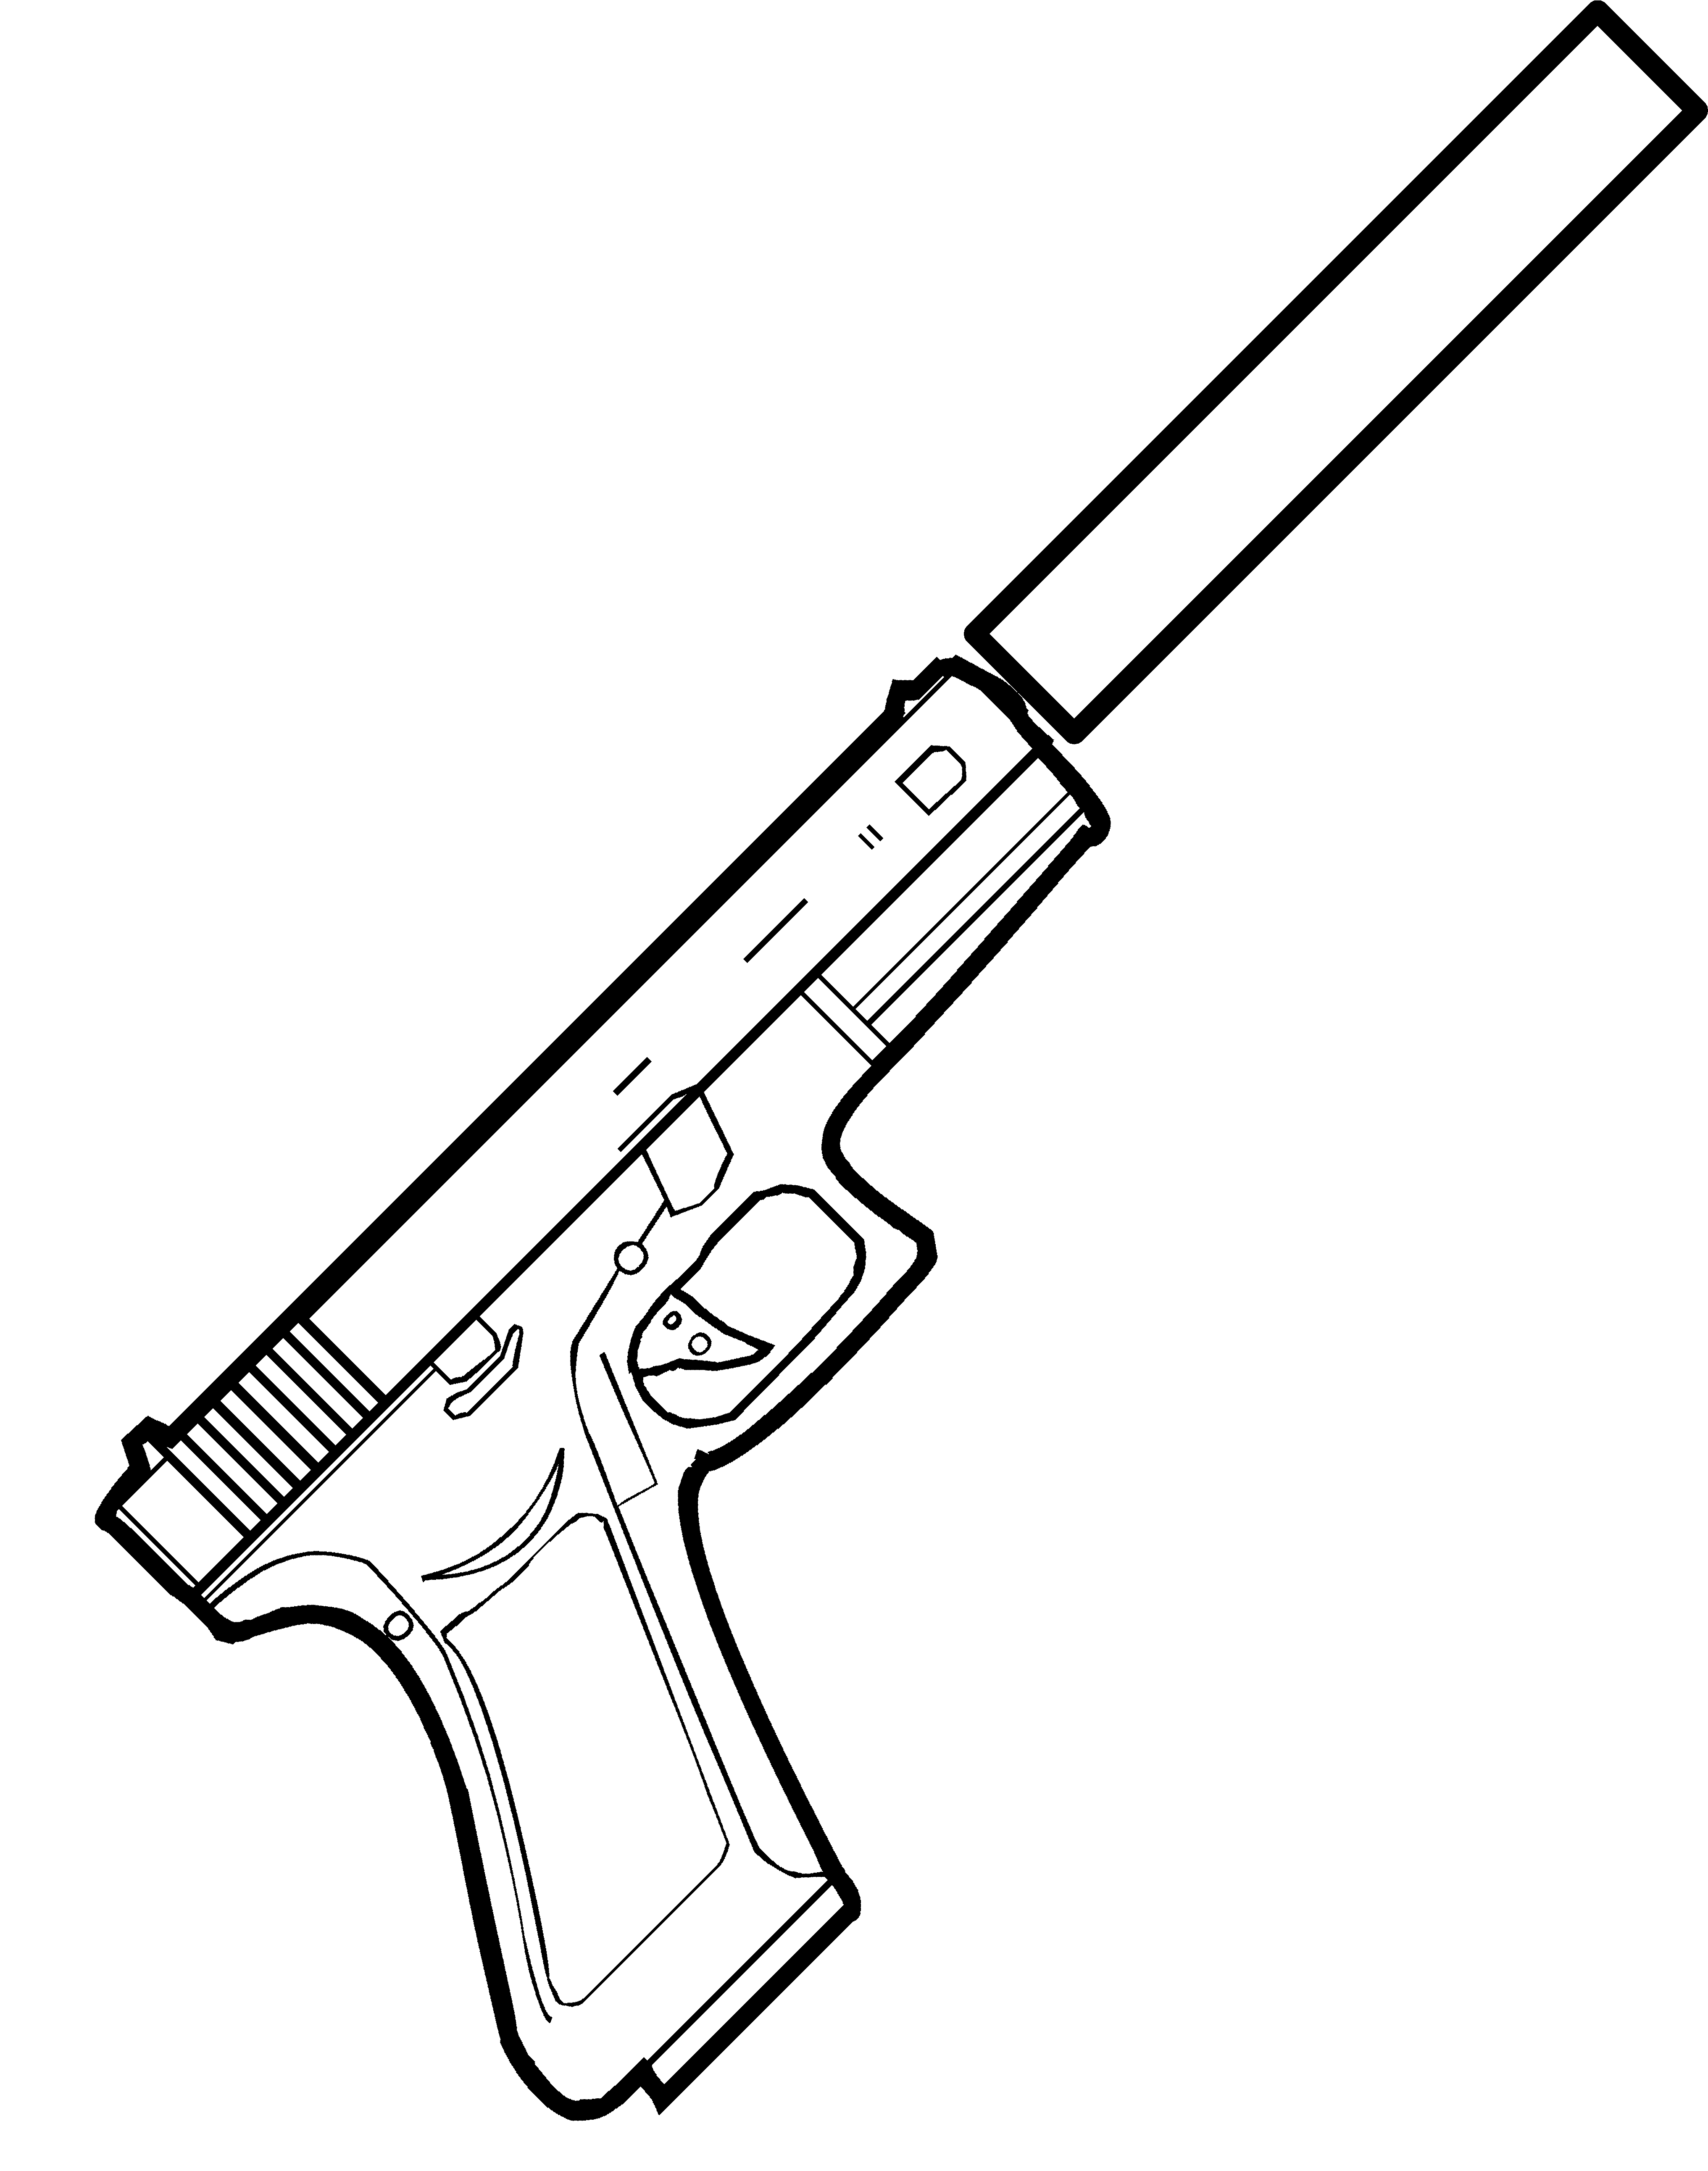
\includegraphics[width=1.5cm]{images/glocksilenced.pdf}}
    }%
  }\\[-1pt]%
}
\foreach \i in {1,...,5} {%
  \foreach \j in {1,2} {%
    \RangedWeaponCard{
      name={Cordite Rifle},
      acc=3,
      damage={6d pi},
      rof=1,
      range={100/1,000},
      bulk=2,
      shots=\scalebox{0.9}[1.0]{30+1(3)},
      rcl=2,
      st=9,
      notes=,
      points=26,
      lc=2,
      weaponpic={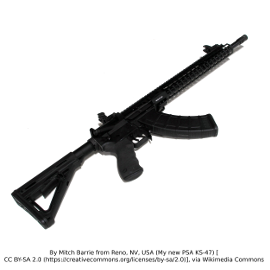
\includegraphics[width=1.9cm]{images/rifle.png}}
    }%
  }\\[-1pt]%
}
\foreach \i in {1,...,5} {%
  \foreach \j in {1,2} {%
    \RangedWeaponCard{
      name={Silenced Cordite Rifle},
      acc=3,
      damage={6d pi},
      rof=1,
      range={100/1,000},
      bulk=2,
      shots=\scalebox{0.9}[1.0]{30+1(3)},
      rcl=2,
      st=9,
      notes=,
      points=27,
      lc=3,
      weaponpic={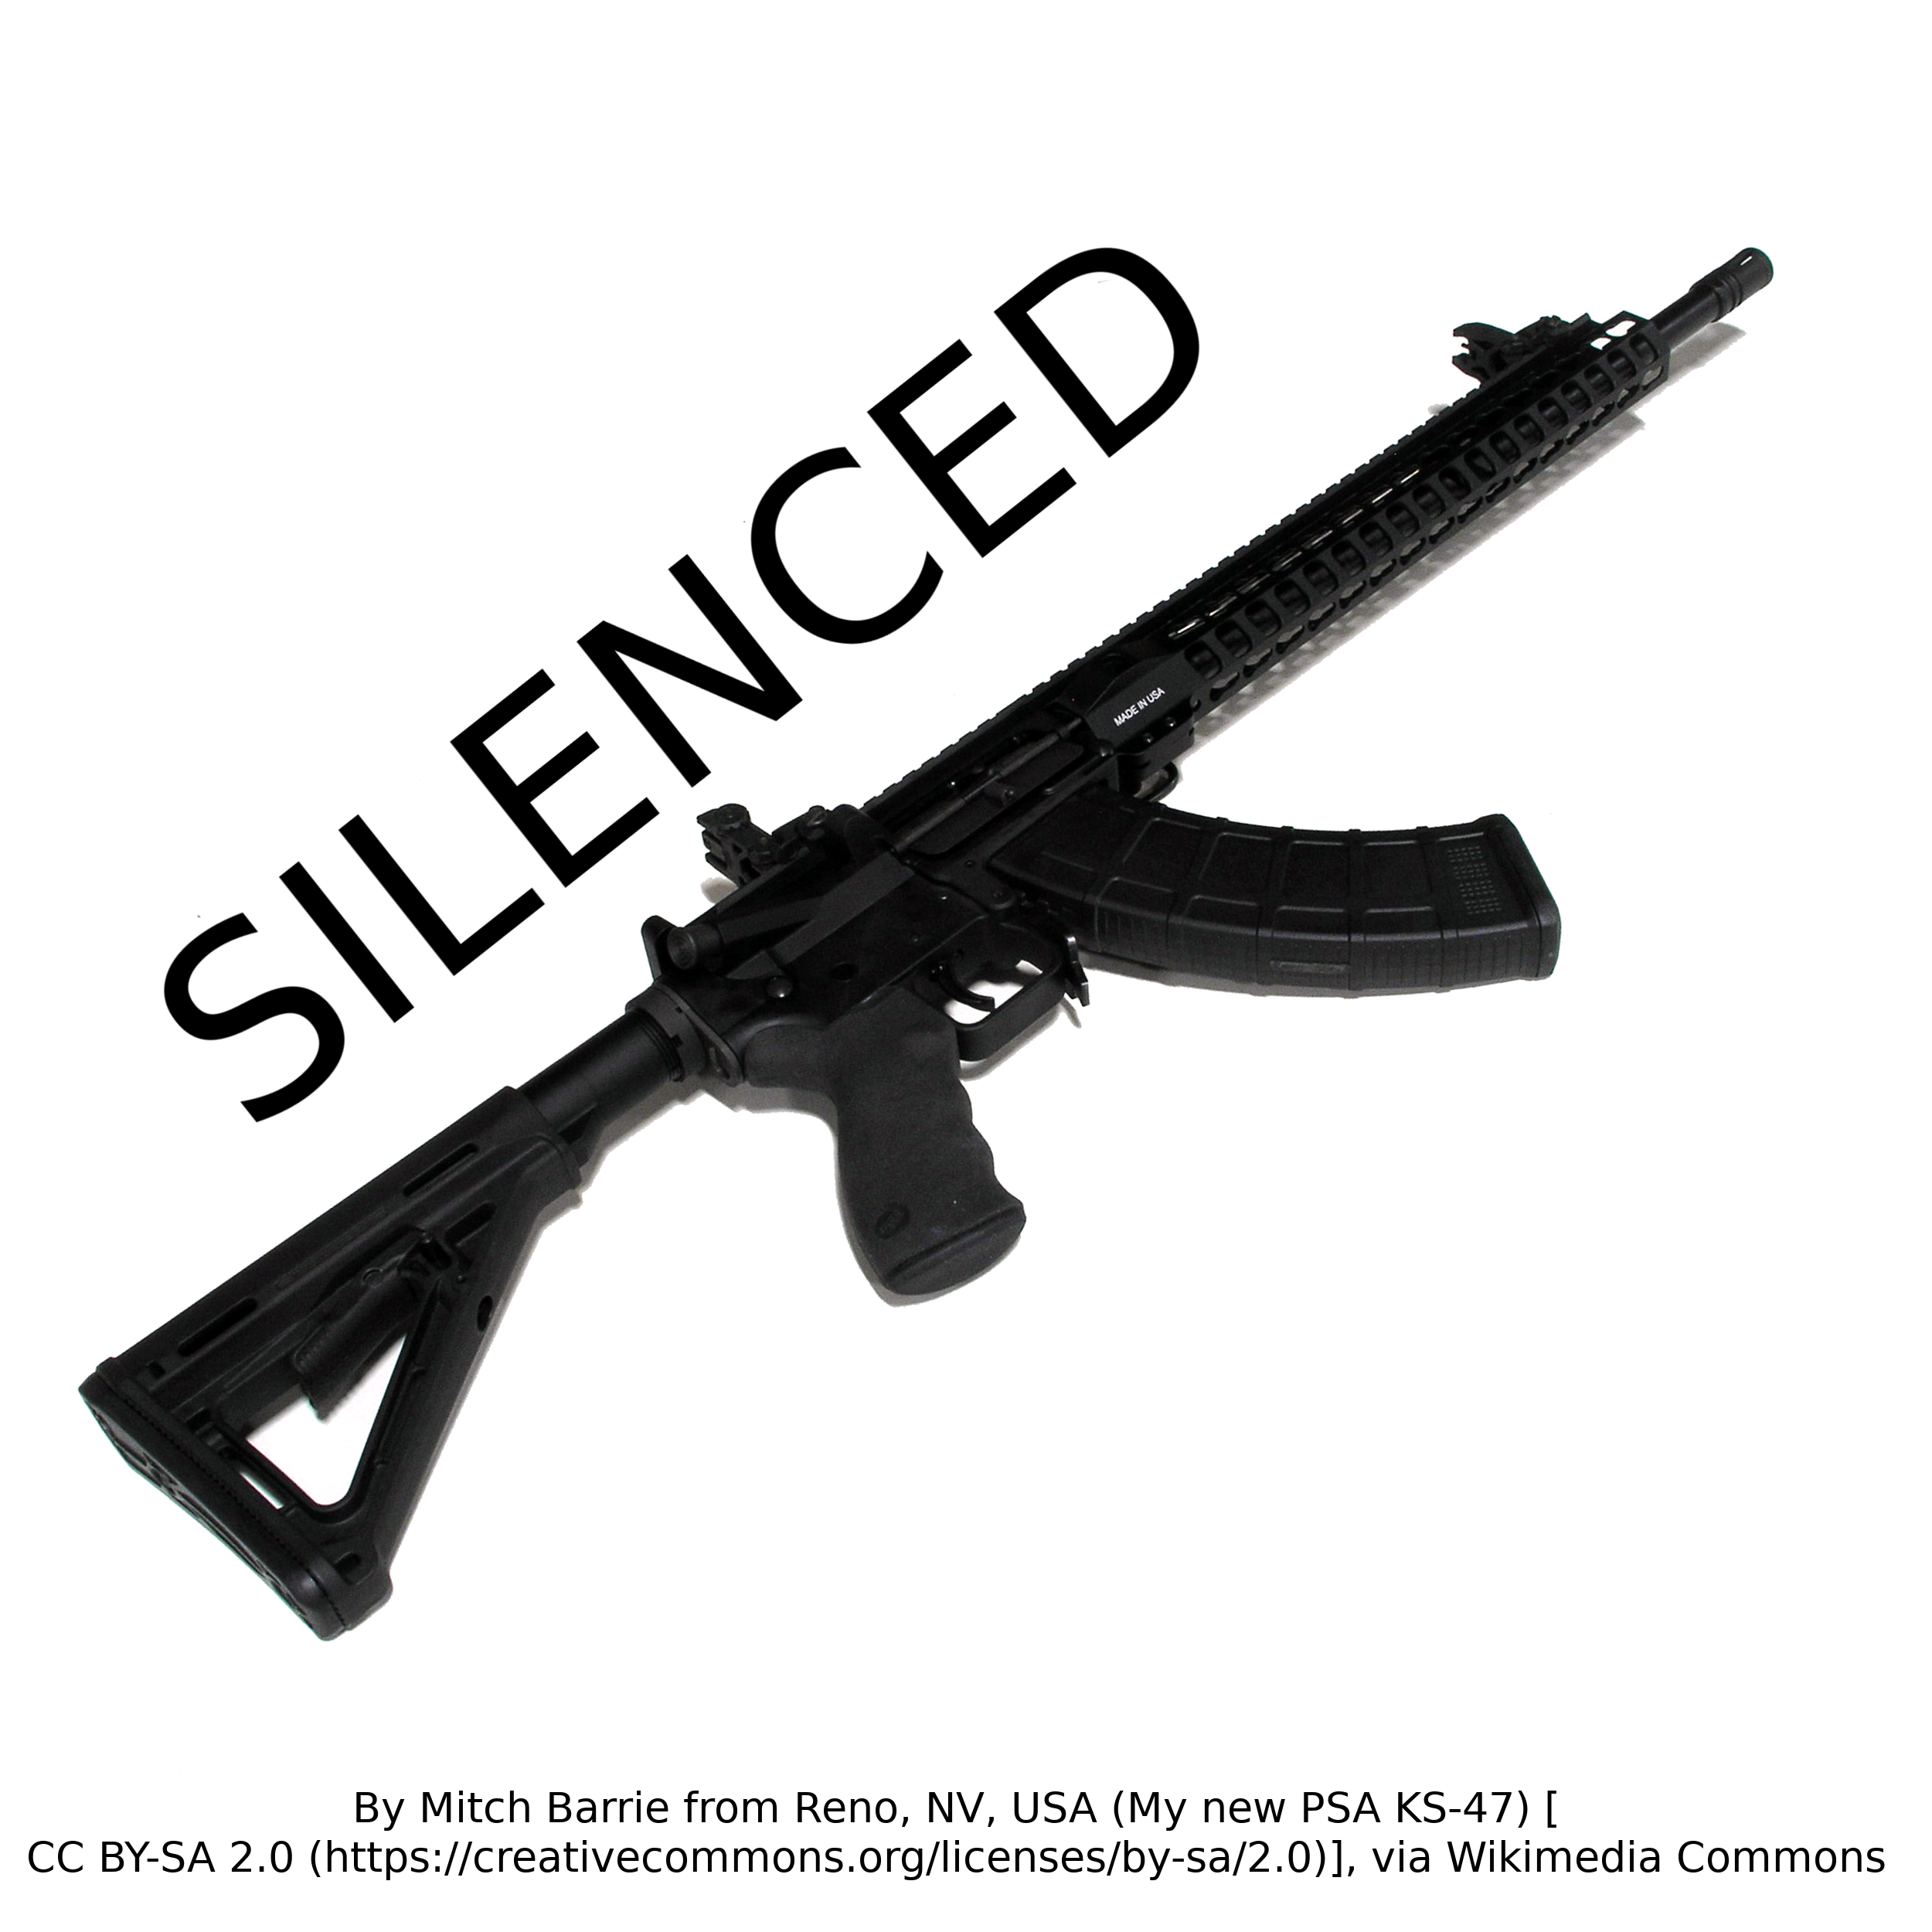
\includegraphics[width=1.9cm]{images/riflesilenced.png}}
    }%
  }\\[-1pt]%
}
\foreach \j in {1,2} {%
  \MeleeWeaponCard{
    name=katana-but-not,
    parry=0,
    damage=1d+2/1d+4,
    reach={\scalebox{0.9}[1.0]{1,2(cut only)}},
    st=8,
    lc=1,
    points=11,
    notes=,
    weaponpic={
\includegraphics[width=1.9cm]{images/katanasword.pdf}}
  }%
}\\[-1pt]
\RangedWeaponCard{
  name={Sling},
  acc=0,
  damage={sw pi},
  rof=1,
  range={6x/10x},
  bulk=-4,
  shots=1(2),
  st=6,
  notes=,
  points=0\raisebox{1ex}{\small *},
  lc=0,
}%
\newpage
\NewDocumentCommand{\ul}{m}{\rule[-2pt]{#1}{0.3pt}}%
\foreach \i in {1,...,10} {%
  \foreach \j in {1,2} {%
    \RangedWeaponCard{
      name=\ul{9.5em},
      damage=\ul{2em},
      acc=\ul{1em},
      rof=\ul{1em},
      range=\ul{4em},
      bulk=\ul{1em},
      shots=\ul{2em},
      rcl=\ul{1ex},
      st=\ul{2ex},
      lc=\ul{1ex},
      points=\rule{0pt}{1ex},
      cost=\ul{2em},
      weight=\ul{2em},
      notes=\ul{9.5em}
    }%
  }\\[-1pt]%
}
\foreach \i in {1,...,10} {%
  \foreach \j in {1,2} {%
    \MeleeWeaponCard{
      name=\ul{9.5em},
      parry=\ul{1em},
      damage=\ul{2em},
      reach=\ul{2em},
      st=\ul{2ex},
      lc=\ul{1ex},
      points=\rule{0pt}{1ex},
      cost=\ul{2em},
      weight=\ul{2em},
      notes=\ul{9.5em}
    }%
  }\\[-1pt]%
}
\end{document}

%%% Local Variables:
%%% mode: latex
%%% TeX-master: "main"
%%% End:
